\documentclass{article}
\usepackage{tikz}
\usepackage{geometry}
\usepackage{amsmath}
\usepackage{wasysym}
\usetikzlibrary{mindmap}
\geometry{a2paper, landscape, margin=2in}

\begin{document}
\begin{figure}\centering

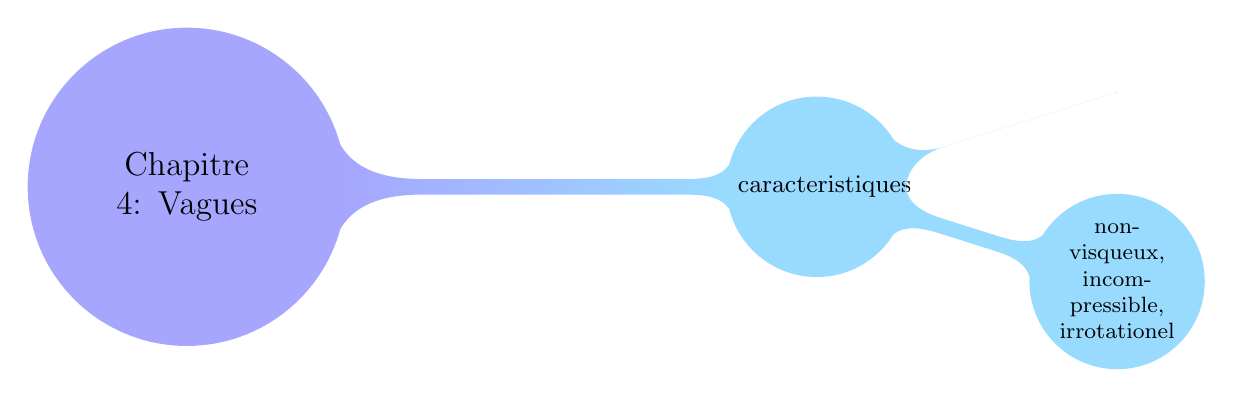
\begin{tikzpicture}[mindmap, grow cyclic, every node/.style=concept,concept color=blue!35,
	level 1/.append style={level distance=8cm,sibling angle=40,every child/.style={concept color=blue!35!cyan!40}},
	level 2/.append style={level distance=4cm,sibling angle=35},
    level 3/.append style={level distance=3cm,sibling angle=45}
    ]

\node {Chapitre 4: Vagues}
    child { node {caracteristiques}
        child [concept]{node[concept] {non-visqueux, incompressible, irrotationel}
        }
    child
    }

;


\end{tikzpicture}
\end{figure}
\end{document}